\begin{figure}[H]
    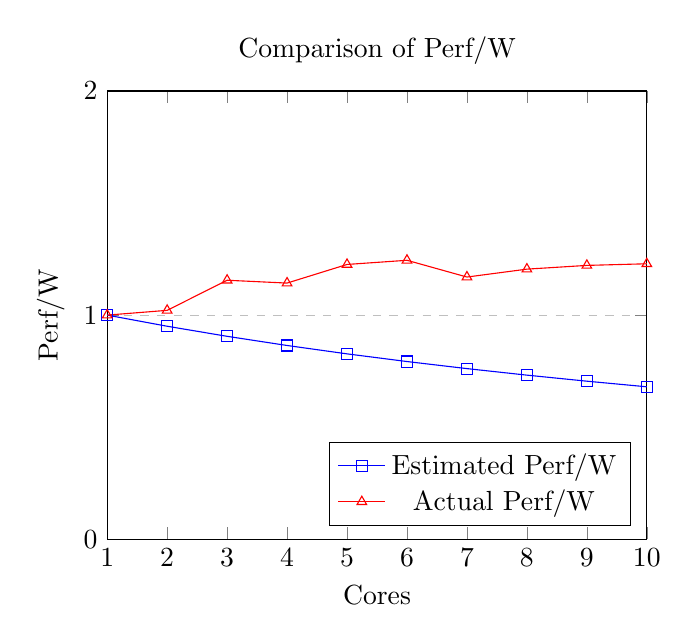
\begin{tikzpicture}
    \begin{axis}[
        title={Comparison of Perf/W},
        xlabel={Cores},
        ylabel={Perf/W},
        xmin=1, xmax=10,
        ymin=0, ymax=2,
        xtick={1,2,3,4,5,6,7,8,9,10},
        ytick={0,1,2},
        legend pos=south east,
        ymajorgrids=true,
        grid style=dashed,
    ]
    
    \addplot[
        color=blue,
        mark=square,
        ]
        coordinates {
        (1,1)(2,0.9503490384)(3,0.9053952915)(4,0.8645022976)(5,0.8271436113)(6,0.7928800172)(7,0.7613421813)(8,0.7322172846)(9,0.7052386117)(10,0.6801773589)
        };
        \addlegendentry{Estimated Perf/W}
    
    \addplot[
        color=red,
        mark=triangle,
        ]
        coordinates {
        (1,1)(2,1.0212549623)(3,1.1555507206)(4,1.1429041218)(5,1.2259919173)(6,1.2445716215)(7,1.1698306081)(8,1.2050913406)(9,1.2217677847)(10,1.2289907387)
        };
        \addlegendentry{Actual Perf/W}
    
    \end{axis}
    \end{tikzpicture}
    \caption{A comparison on the estimated Perf/W from Amdahl's extended law and the actual Perf/W for 3DM on DUT 2}\label{fig:amdahlsExtPerfW}
\end{figure}
